\documentclass[rnd]{mas_proposal}
% \documentclass[thesis]{mas_proposal}
\usepackage{caption}
\usepackage[utf8]{inputenc}
\usepackage{amsmath}
\usepackage{amsfonts}
\usepackage{amssymb}
\usepackage{graphicx}
%\usepackage{enumitem}
\usepackage[british]{babel}

\title{Feature Detection and analysis\\in digital twin of thermoplastic UD tapes }
\author{Somesh Devagekar}
\supervisors{Prof. Dr Paul G.Plöger\\Klaus Wolf \\ Third Supervisor}
\date{MAY 2019}

\thirdpartylogo{Fraunhofer.jpg}











\begin{document}
\newcommand{\SubItem}[1]{
    {\setlength\itemindent{15pt} \item[-] #1}
}

\maketitle

\pagestyle{plain}

\chapter{Introduction}
\begin{figure}
\centering
\begin{minipage}{.4\textwidth}
  \centering
  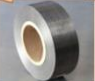
\includegraphics[width=0.4\linewidth]{tape.png}
  \captionof{figure}{UD Tape}
  \label{fig:test1}
\end{minipage}%
\begin{minipage}{.5\textwidth}
  \centering
  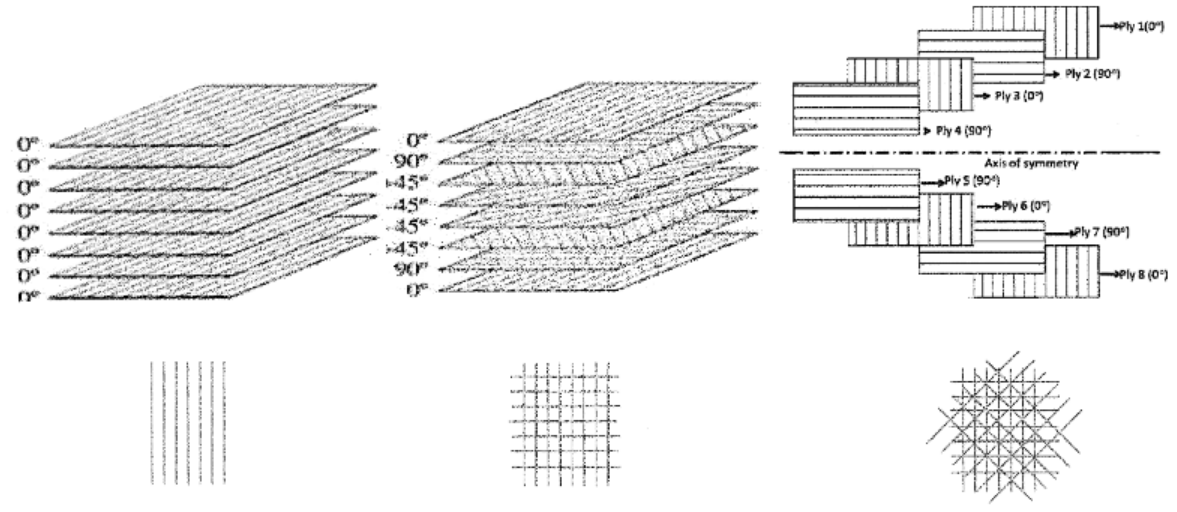
\includegraphics[width=1\linewidth]{stacking.png}
  \captionof{figure}{stacking of UD tapes}
  \label{fig:test2}
\end{minipage}
\end{figure}
    Unidirectional tapes (Fig-1.1) have reinforced fibers which are made of carbon or glass and these tapes are placed on each other in such a way that they can adapt the component load, thereby increasing the overall load bearing capacity(Fig-1.2)[1].\\
\indent    A digital replica(digital twin), creates a representation of the physical entity and serves as an important aspect in optimizing systems and process(Fig-3). To achieve this
continuous digitization relevant tape characteristics are needed to be analyzed with the help of cognitive sensors. Some of the characteristics observed are thickness profile, local fiber and pore content, local deviations from fiber orientation. Using this domain knowledge, we can predict material grades and accordingly adjust parameters along the supply chain.\\
 \indent   Machine learning approaches model these tape characteristics as an ideal regression prediction model. Some of these algorithms include linear and logistic regression, neural networks, convolution neural networks, Gaussian process and so on. The tasks of these algorithms involve classification, identification and appropriate segmentation.\\
\indent With the digital transformation under "Industry 4.0" or "IIOT" and wide spread of digital twins, much of the focus is on leveraging machine learning algorithms to understand and deduce the final product itself. Gartner predicts by 2020 more than 20 billion networked sensors will be used in industrial environments[2], enabling fundamental knowledge about material behavior, products and processes. However, digital twins can also be used in real time capability to influence material conditions in the intermediate and end product stages to gain precise mapping and tracking of composite structures.  \\


\section{Problem Statement}
  \indent  UD tapes have incredible load bearing capacity, particularly due to their complex
and heterogeneous microstructure. These tapes are influenced by manufacturing
process in the production of semi finished products and finished structural
component. As a result it provides tremendous challenge to achieve continuous
digitization of the entire production process. Thus with the help of a digital profile of a component, it is advantageous to detect component weakening flaws each time they arise. For example, due to material fluctuations or the use of recycled material,the fiber orientation and the pore content in the composite can be addressed. \\
  \indent  To achieve this continuous digitization of the process, a joint use of material and
process data across all process stages is needed for example in quality assurance.
Defects (wrong fiber orientation, pores, dry zones, foreign bodies) can be detected,
classified and accordingly measured in the semi finished component. With both optical, acoustic and electrical eddy current sensors data, a direct correlation can be made towards the structural change in the production process. As a part of the digital twin, this research aims at understanding crucial quality features that contribute towards a structural change of the composite, in a data driven quality assurance control production process.\\

\chapter{Related Work}
\section{Section 1}
Most of the current approaches in digital manufacturing are limited to using data from manufacturing sectors and the end product. Intermediate tracking and locally mapping of process influenced materials has not being implemented in digital twins.  \\
\indent Some of the testing methods in fiber reinforced are usually comprised of non-destructive evaluation techniques[3]. Here the authors formulate the complexity of having a quality control mechanism for mis-orientations in fibers.\\
\indent To monitor the structural health of a composite, prognosis at an early stage is important[4]. Here the authors have said that since damage analysis is innefficient, a framework for understanding delimination caused in composite fibers has to be modeled.\\
\indent With the use of simulation properties from different tools as domain knowledge, we can reason out the vast space of composite structure data , into learning algorithms to detect features that maps input variables to a end product.[5]

\section{Section 2}
Implementation of machine learning stratergies on understanding the composite structure in a semi finished product has not bee tapped yet. However most of investigation lies in understanding the contributing features at the end product itself for example non-destructive evaluation.\\
\indent To understand the diversified structure of a composite material it is important to understand the crucial contributing features and not just the delimination size. 



\chapter{Project Plan}

\section{Work Packages}
The bare minimum will include the following packages:
\begin{enumerate}
    \item[WP1] Literature Search
        \SubItem{Literature on UD tapes}
        \SubItem{Literature on generalised feature extraction frameworks}
        \SubItem{Literature on feature extraction in composites}
    \item[WP2] Data defination
     \SubItem{Prioritization of raw input data}
     \SubItem{Feature defination}
     \SubItem{Corelation of dataset to literature review}
    \item[WP3] Experimentation
    \SubItem{Exploratory data analysis}
    \SubItem{Sample feature extraction and feature engineering model}
    \SubItem{Proposed feature transformation model}
    \SubItem{Proposed feature selection model}
    \item[WP4] Project report
    \SubItem{Achieved progress summary}
    \SubItem{Overall project outline}
\end{enumerate}

\section{Milestones}

\begin{enumerate}
    \item[M1] Literature search(UD tapes and feature extraction)
    \item[M2] Literature analysis and data defination
    \item[M3] Experiment defination
    \item[M4] Experiment analysis
    \item[M5] Project Report
 \end{enumerate}
\vspace{50px}
\section{Project Schedule}

\begin{figure}[h!]
    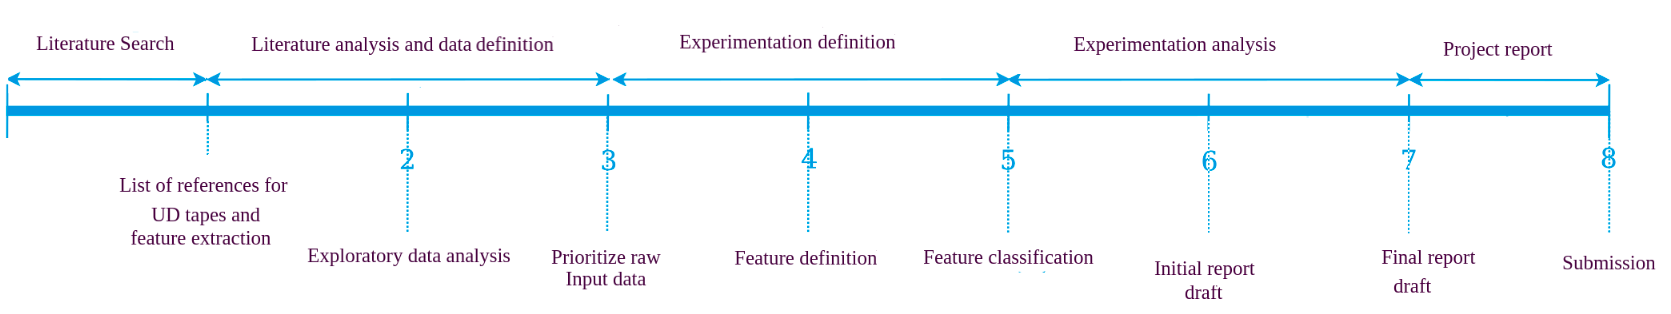
\includegraphics[width=1\textwidth]{timeschedule}
    \caption{}
    \label{}
\end{figure}
\pagebreak
\section{Deliverables}
\subsection{Minimum Viable}
\begin{itemize}
    \item Survey analysis
    \item Evaluation of feature extraction technique
\end{itemize}

\subsection{Expected}
\begin{itemize}
    \item Analysis of the state of the art
\end{itemize}

\subsection{Desired}
\begin{itemize}
    \item Appropriate classification of UD tapes
\end{itemize}


\nocite{*}

\bibliographystyle{plainnat} % Use the plainnat bibliography style
\bibliography{bibliography.bib} % Use the bibliography.bib file as the source of references





\end{document}
